%!TEX root = ../Chimica.tex
\documentclass[11pt,oneside]{scrbook}

% ---------- LINGUA & CODIFICA ----------
\usepackage[italian]{babel}
\usepackage[T1]{fontenc}
\usepackage[utf8]{inputenc}
\usepackage{csquotes}

% ---------- TIPOGRAFIA CONSIGLIATA ----------
\usepackage{lmodern}     % font semplice e diffuso
\usepackage{microtype}   % micro-tipografia, migliore resa

% ---------- FIGURE IN TIKZ -----------

\usepackage{tikz}
\usetikzlibrary{arrows.meta, patterns, decorations.markings, decorations.pathmorphing, calc, positioning}
\usepackage{amsmath, amssymb, bm}
\usepackage{circuitikz}

% --- stili e macro (nel preambolo) ---
\tikzset{
  boccola/.style={circle,draw,thick,fill=white,inner sep=0pt,minimum size=5pt},
  cavo/.style={thick,rounded corners},
  morsetto/.style={font=\footnotesize,above=3pt},
  etichetta/.style={font=\small}
}
% quattro boccole equispaziate: b1 b2 = avv. interno, b3 b4 = avv. esterno
\newcommand{\boccole}{%
  \foreach \i in {1,2,3,4} {\node[boccola] (b\i) at (1.5*\i,0) {};}%
}
% cavo tra due boccole; argomento opzionale = looseness
\newcommand{\cavo}[3][1.3]{\draw[cavo] (#2) to[out=-70,in=-110,looseness=#1] (#3);}

% Stile coerente con le immagini a colori
\definecolor{posred}{RGB}{239,130,140}   % rosa-rosso per cariche positive
\definecolor{negblue}{RGB}{120,190,230}  % azzurro per cariche negative
\definecolor{ered}{RGB}{227,35,35}       % rosso vivo per i vettori E
\definecolor{surfblue}{RGB}{205,230,245} % azzurro chiaro per la superficie
\definecolor{gray60}{gray}{0.55}
\definecolor{blobpink}{RGB}{245,205,190} % colore del corpo esteso
\definecolor{cubecol}{RGB}{235,190,170}
\definecolor{charge}{RGB}{245,175,120}      % arancione chiaro delle cariche
\definecolor{matpink}{RGB}{245,210,195}     % superficie superiore del materiale
\definecolor{matpinkdk}{RGB}{225,175,155}   % fianco laterale
\definecolor{loopblue}{RGB}{90,130,200}     % anelli di corrente
\definecolor{mred}{RGB}{227,35,35}          % vettore M
\definecolor{surrfblue}{RGB}{190,215,235}   % regione chiusa C (riempimento)
\definecolor{surfedge}{RGB}{80,120,170}     % bordo della curva C
\definecolor{ghost}{RGB}{140,140,140}       % traslazione (tratteggiata)
\definecolor{vred}{RGB}{227,35,35}          % vettori v



% ---------- GEOMETRIA PAGINA ----------
% Scegli *una* delle due geometrie qui sotto.
% (1) Impostazioni consigliate per A4 (Italia) con ampio margine esterno:
\usepackage[
  a4paper,
  top=24mm,
  bottom=28mm,
  inner=28mm,   % margine interno (verso rilegatura)
  outer=50mm,   % margine esterno: ampio per le note a margine
  heightrounded
]{geometry}
\setlength{\headheight}{17pt} % evita sovrapposizioni con l'header
\setlength{\headsep}{6mm}     % distanza tra header e corpo


% (2) Se vuoi replicare il formato del PDF caricato (US Letter 8.5x11"):
% \usepackage[
%   letterpaper,
%   top=25mm,
%   bottom=30mm,
%   inner=30mm,
%   outer=55mm,
%   heightrounded
% ]{geometry}

% ---------- HEADER/FOOTER ----------
\usepackage{fancyhdr}
\pagestyle{fancy}
\fancyhf{} % pulisci

% intestazione: solo titolo del capitolo (sinistra), pagina a destra
\fancyhead[L]{\nouppercase{\leftmark}}
\fancyfoot[R]{\thepage}

\renewcommand{\headrulewidth}{0.4pt}
\renewcommand{\footrulewidth}{0pt}

\fancypagestyle{plain}{%
  \fancyhf{}
  \fancyfoot[R]{\thepage}
  \renewcommand{\headrulewidth}{0pt}
}

% ---------- STRUMENTI DI STRUTTURA ----------
\setcounter{secnumdepth}{3}
\setcounter{tocdepth}{2}
\usepackage{titlesec}

% --- Titoli puliti ---
% Capitolo
\titleformat{\chapter}[display]
  {\normalfont\huge\bfseries}
  {\thechapter}{1ex}{}
\titlespacing*{\chapter}{0pt}{-0.5em}{1.5ex}

% Capitolo
\titleformat{\chapter}[display]
  {\normalfont\huge\bfseries}
  {\thechapter}{1ex}{}
\titlespacing*{\chapter}{0pt}{1.5ex}{1.5ex}

% Sezione
\titleformat{\section}
  {\normalfont\Large\bfseries}
  {\thesection}{1em}{}

% Sottosezione
\titleformat{\subsection}
  {\normalfont\large\bfseries}
  {\thesubsection}{0.8em}{}

% SOTTO-sottosezione  <--- AGGIUNGI QUESTO BLOCCO
\titleformat{\subsubsection}
  {\normalfont\normalsize\bfseries}
  {\thesubsubsection}{0.8em}{}
\titlespacing*{\subsubsection}{0pt}{0.8ex}{0.4ex}

% Paragrafo (run-in: titolo in grassetto sulla stessa riga del testo)
\titleformat{\paragraph}[runin]
  {\normalfont\normalsize\bfseries}
  {}{0pt}{}[.]
\titlespacing*{\paragraph}{0pt}{1ex}{0.5em}

% ---------- PAGINA SEPARATRICE ----------
\newcommand{\partpage}[1]{%
  \cleardoublepage          % vai a pagina nuova (pari se oneside)
  \thispagestyle{empty}     % niente header/footer
  \null\vfill               % spazio verticale elastico sopra
  \begin{center}
    {\Huge\bfseries #1}
  \end{center}
  \vfill\null               % spazio verticale elastico sotto
  \cleardoublepage          % lascia la pagina successiva libera
}

% ---------- AMBIENTI UTILI ----------
\usepackage{amsmath,amssymb,amsthm}
\usepackage{graphicx}
\usepackage[hidelinks]{hyperref}
\usepackage{xcolor}
\usepackage{tcolorbox}
\usepackage{subcaption}
\usepackage{booktabs}
\usepackage{multirow}
\usepackage[version=4]{mhchem}   % per \ce{}
\usepackage{siunitx}             % per \SI{} e \si{}


% ---------- NOTE A MARGINE (parole-chiave/sidenote) ----------
% Definiamo un comando comodo e graficamente coerente:
\newcommand{\mkeyword}[1]{%
  \marginpar{\raggedright\footnotesize\emph{#1}}%
}

% Se preferisci le note a sinistra, attiva la riga seguente:
% \reversemarginpar

% ---------- PARAGRAFI E SPAZI ----------
\setlength{\parindent}{0.8em}  % rientro tradizionale
\setlength{\parskip}{0.25em}   % piccolo spazio extra tra paragrafi

%----------- COMANDI AGGIUNTIVI -----------
% --- Comando per vettori colonna di lunghezza variabile ---

\newcommand{\colvec}[1]{%
  \begin{pmatrix}
    #1
  \end{pmatrix}%
}

\renewcommand{\Re}{\operatorname{Re}}
\renewcommand{\Im}{\operatorname{Im}}

\newcommand{\FIG}[1]{
  \begin{figure}[h]
    \centering
    \includegraphics[width=0.4\linewidth]{figure/image#1.png}
    \caption{}
    \label{}
  \end{figure}
}

\newcommand{\eps}{\varepsilon}

\theoremstyle{definition}
\newtheorem{definizione}{Definizione}[chapter]
\newtheorem{esempio}[definizione]{Esempio}

\theoremstyle{remark}
\newtheorem{osservazione}[definizione]{Osservazione}

\theoremstyle{plain}
\newtheorem{teorema}[definizione]{Teorema}
\newtheorem{proposizione}[definizione]{Proposizione}

% % ---------- BIBLIOGRAFIA ----------
% \usepackage[backend=biber,style=numeric,sorting=nyt]{biblatex}
% \addbibresource{chapters/bibliografia.bib}

% ---------- FRONTESPIZIO ----------
\title{\textbf{Esperienze di Laboratorio 2}}
\author{Roberto Riccucci}
\date{}

\publishers{
  Email: \text{roberto.riccucci1304@gmail.com} \\
  Versione: v0.1
}



\begin{document}

\frontmatter

\newgeometry{
    top=24mm,
    bottom=28mm,
    left=39mm,
    right=39mm,
    heightrounded
}
\begin{titlepage}
    \centering

    \makebox[\textwidth][c]{\Huge\bfseries Chimica Generale \par}

    \vspace{1cm}

    \makebox[\textwidth][c]{\Large Roberto Riccucci \par}

    \vspace{1.5cm}

    \makebox[\textwidth][c]{\rule{0.8\textwidth}{0.4pt}}

    \vspace{0.7cm}

    \makebox[\textwidth][c]{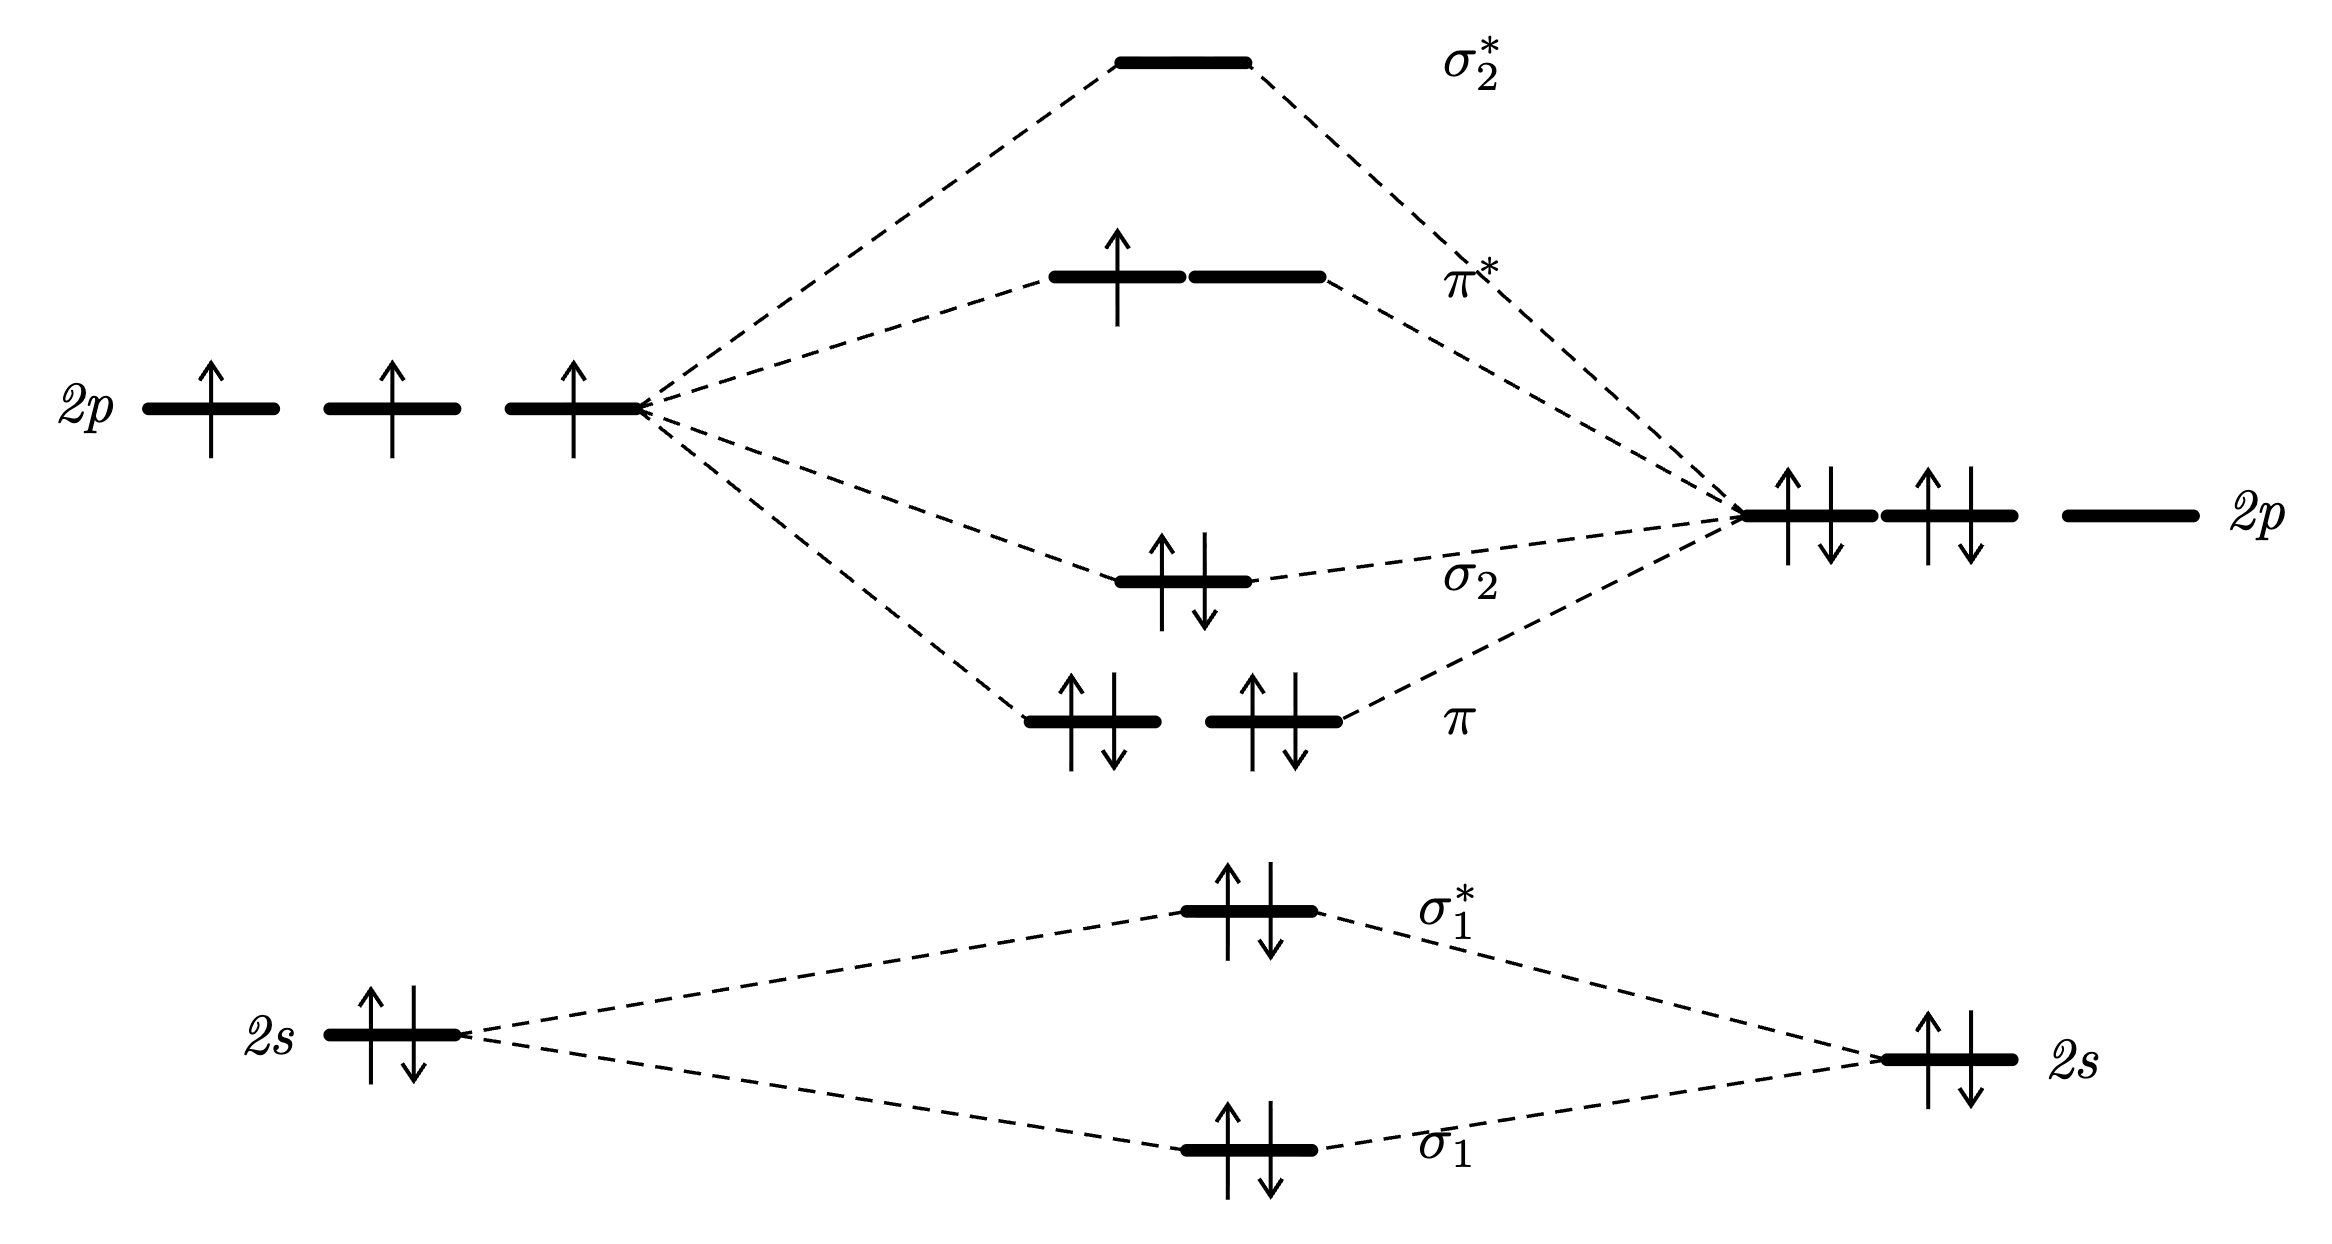
\includegraphics[width=0.7\textwidth]{foto/mo.png}}

    \vspace{0.7cm}

    \makebox[\textwidth][c]{\rule{0.8\textwidth}{0.4pt}}

    \vfill

    \makebox[\textwidth][c]{\large Versione v0.1 \par}
    \makebox[\textwidth][c]{\small robertoriccucci1304@gmail.com \par}

\end{titlepage}
\restoregeometry

\tableofcontents

%\input{Esperienze/Manuali.tex}

\mainmatter

\chapter{Teoria atomica}

La chimica diventa una scienza quantitativa nella seconda metà del XVIII secolo, quando l'introduzione sistematica della bilancia nello studio delle trasformazioni della materia permette di sostituire le descrizioni qualitative con misure di massa. 
Le regolarità osservate in queste misure prendono il nome di \emph{leggi ponderali}: sono leggi empiriche, dedotte dai dati sperimentali prima che di esse esistesse una spiegazione teorica.
 
Il loro interesse non è soltanto storico. Come vedremo, esse costituiscono l'evidenza sperimentale su cui Dalton fonda la teoria atomica: sono cioè il ponte tra ciò che si misura in laboratorio e l'ipotesi che la materia sia costituita da particelle discrete.
 
\subsection{Legge di conservazione della massa}
 
Il primo a condurre in modo sistematico esperimenti quantitativi sulle trasformazioni della materia è Antoine-Laurent Lavoisier, intorno al 1789.
 
\begin{definizione}[Legge di Lavoisier]
    In una reazione chimica che avvenga in un sistema chiuso la massa \mkeyword{legge di conservazione della massa} complessiva non varia: la somma delle masse dei reagenti è uguale alla somma delle masse dei prodotti.
\end{definizione}
 
L'esperimento decisivo riguarda la calcinazione dei metalli. Riscaldando il mercurio in un recipiente chiuso si osserva la formazione di un ossido rosso, e il solido prodotto pesa \emph{più} del metallo di partenza. 
L'apparente violazione della legge si risolve osservando che l'aria contenuta nel recipiente diminuisce di volume: l'incremento di massa del solido è esattamente pari alla massa di aria consumata.
 
La condizione di sistema chiuso è essenziale. Nelle combustioni condotte all'aria aperta parte dei prodotti si disperde in fase gassosa, ed è proprio questo che aveva a lungo mascherato la conservazione della massa, favorendo la teoria del flogisto.
 
\subsection{Legge delle proporzioni definite}
 
Stabilito che la massa si conserva, il passo successivo consiste nel chiedersi in quali rapporti gli elementi si combinino. La risposta è dovuta a Joseph-Louis Proust (1799).
 
\begin{definizione}[Legge di Proust]
    Un composto puro contiene sempre gli stessi elementi combinati nelle \mkeyword{legge delle proporzioni definite} medesime proporzioni in massa, indipendentemente dal metodo con cui è stato preparato e dalla sua provenienza.
\end{definizione}
 
Una conseguenza importante di questa legge è che se si fanno reagire i due elementi in proporzioni diverse da quella caratteristica, l'eccesso rimane semplicemente inalterato a fine reazione: è il concetto di \emph{reagente limitante}.
 
\subsection{Legge delle proporzioni multiple (o di Dalton)}
 
Le prime due leggi descrivono un singolo composto per volta. Il contributo di John Dalton (1803) consiste nel confrontare fra loro composti \emph{diversi} formati dalla stessa coppia di elementi.
 
\begin{definizione}[Legge di Dalton]
    Quando due elementi si combinano fra loro formando composti differenti, \mkeyword{Legge di Dalton} le masse di uno dei due elementi che si combinano con una massa fissata dell'altro stanno tra loro in un rapporto esprimibile mediante numeri interi piccoli.
\end{definizione}
 
In formule, fissata la massa $m_A$ dell'elemento $A$ e dette $m_B^{(1)}$ e $m_B^{(2)}$ le masse dell'elemento $B$ nei due composti,

\begin{equation}
    \frac{m_B^{(1)}}{m_B^{(2)}} = \frac{p}{q}, \qquad p,q \in \mathbb{N} \ \text{piccoli}
    \label{eq:dalton}
\end{equation}

La \eqref{eq:dalton} è la più profonda delle leggi ponderali, perché non si limita a descrivere una regolarità: ne suggerisce la causa.
 
Se la materia fosse un continuo indefinitamente divisibile, non vi sarebbe alcun motivo per cui i rapporti debbano risultare razionali con numeratore e denominatore piccoli; ci si attenderebbero valori arbitrari. 
L'osservazione che i rapporti sono invece sempre semplici trova spiegazione immediata assumendo che ciascun elemento sia costituito da particelle discrete e indivisibili, tutte identiche fra loro, che si combinano in numero intero.
Passare da $PCl_3$ a $PCl_5$ significa aggiungere esattamente due atomi di cloro: non è possibile aggiungerne una frazione, ed è per questo che il rapporto è $5:3$ e non un numero irrazionale qualsiasi.
 
\subsection{Principio di Avogadro}
 
Le leggi precedenti riguardano le masse. Con lo studio delle reazioni fra gas emerge una regolarità di natura diversa, relativa ai volumi, enunciata da Amedeo Avogadro nel 1811.
 
\begin{definizione}[Principio di Avogadro]
    Volumi uguali di gas diversi, misurati nelle medesime condizioni di \mkeyword{principio di Avogadro} temperatura e pressione, contengono lo stesso numero di molecole.
\end{definizione}
 
L'enunciato è coerente con l'equazione di stato dei gas ideali

\begin{equation}
    pV = nRT
    \label{eq:gasideali}
\end{equation}

nella quale, fissati $p$, $V$ e $T$, resta determinato $n$ senza alcun riferimento alla natura chimica del gas. 
È un fatto notevole: il comportamento di un gas ideale dipende dal \emph{numero} di particelle e non dal \emph{tipo}.

\newpage

\section{Modello atomico di Thomson}

Solamente tra il XIX e XX secolo si inziò a interessarsi della conformazione degli atomi. Uno strumento fondamentale a questo scopo fu il tubo di Crookes\mkeyword{tubo di Crookes} (o tubo a raggi catodici), il quale fu creato per vedere se dentro il metallo ci fosse qualcosa in grado di reagire a un campo elettrico. \\

Il tubo di Crookes è un particolare tubo a vuoto di vetro, a forma di ampolla, che presenta due elettrodi: un anodo e un catodo.\\

\begin{tikzpicture}[
    line cap=round,
    line join=round,
    vetro/.style     = {line width=0.6pt},
    elettrodo/.style = {line width=1.2pt},
    filo/.style      = {line width=0.5pt},
    raggio/.style    = {line width=0.4pt, -{Straight Barb[length=2.2pt,width=2.6pt]}},
    etichetta/.style = {font=\footnotesize, inner sep=1.5pt}
]

% ---- ampolla di vetro ----
\draw[vetro]
    (-4.2,0) .. controls (-4.2,1.05) and (-3.5,1.25) .. (-2.6,1.25)
    -- (2.6,1.25)
    .. controls (3.5,1.25) and (4.2,1.05) .. (4.2,0)
    .. controls (4.2,-1.05) and (3.5,-1.25) .. (2.6,-1.25)
    -- (-2.6,-1.25)
    .. controls (-3.5,-1.25) and (-4.2,-1.05) .. (-4.2,0);

% ---- bocchettone per il vuoto ----
\draw[vetro] (-0.30,1.24) -- (-0.30,1.80) -- (-0.44,1.80);
\draw[vetro] ( 0.30,1.24) -- ( 0.30,1.80) -- ( 0.44,1.80);
\draw[filo,-{Straight Barb[length=3pt]}] (0,1.95) -- (0,2.45);
\node[etichetta,anchor=west] at (0.20,2.30) {alla pompa da vuoto};

% ---- catodo ----
\draw[elettrodo] (-3.55,-0.62) -- (-3.55,0.62);
\draw[filo] (-3.55,0) -- (-4.85,0);
\node[etichetta,anchor=east] at (-4.95,0) {$-$};
\node[etichetta,anchor=north] at (-3.55,-0.75) {catodo};

% ---- anodo ----
\draw[elettrodo] (3.30,-0.50) -- (3.30,0.50);
\draw[filo] (3.30,0) -- (4.85,0);
\node[etichetta,anchor=west] at (4.95,0) {$+$};
\node[etichetta,anchor=north] at (3.30,-0.62) {anodo};

% ---- diaframma con fenditura ----
\draw[elettrodo] (-1.55,-1.05) -- (-1.55,-0.22);
\draw[elettrodo] (-1.55, 0.22) -- (-1.55, 1.05);
\node[etichetta,anchor=south] at (-1.55,1.34) {diaframma};

% ---- fascio di raggi catodici ----
\foreach \y in {-0.34,-0.17,0,0.17,0.34}{
    \draw[raggio] (-3.42,\y) -- (-1.70,{0.42*\y});
}
\foreach \y in {-0.14,0,0.14}{
    \draw[raggio] (-1.40,{0.55*\y}) -- (2.00,\y);
}

% ---- croce di Malta ----
\filldraw[fill=white, line width=0.7pt]
    (2.12,-0.14) -- (2.12,-0.44) -- (2.42,-0.44) -- (2.42,-0.14)
    -- (2.72,-0.14) -- (2.72, 0.16) -- (2.42, 0.16) -- (2.42, 0.46)
    -- (2.12, 0.46) -- (2.12, 0.16) -- (1.82, 0.16) -- (1.82,-0.14) -- cycle;
\node[etichetta,anchor=south] at (2.27,0.58) {ostacolo};

% ---- fluorescenza della parete di fondo ----
\foreach \a in {28,42,56,-28,-42,-56}{
    \draw[line width=0.35pt]
        ($(2.6,0)+({1.60*cos(\a)},{1.25*sin(\a)})$) --
        ($(2.6,0)+({1.60*cos(\a)+0.20*cos(\a)},{1.25*sin(\a)+0.20*sin(\a)})$);
}

% ---- ombra proiettata ----
\draw[line width=0.5pt] (3.90,0.46) .. controls (4.00,0.20) and (4.00,-0.20) .. (3.90,-0.46);
\draw[filo] (3.96,-0.36) -- (4.15,-1.30);
\node[etichetta,anchor=north] at (4.15,-1.30) {ombra};

\end{tikzpicture}

\vspace{0.5 cm}

Grazie a questo nel 1897 fu scoperto che quelli che all'epoca erano chiamati raggi catodici (e che oggi sappiamo essere \emph{elettroni}\mkeyword{elettroni}) hanno una carica e una massa e fu trovato anche il rapporto tra queste due quantità ($q/m = 1,76 \cdot 10^8 \ C/g$).

Il valore esatto delle singole quantità fu ottenuto nel 1909 tramite un esperimento condotto da Millikan\footnote{L'esperimento andava a cercare l'equilibrio di gocce d'olio caricate per strofinio soggette a un campo elettrico e alla forza di gravità}.\\

Dal confronto con il rapporto analogo dello ione idrogeno, noto dall'elettrolisi, si ricava inoltre che la massa dell'elettrone è circa $1800$ volte più piccola di quella dell'atomo di idrogeno. Poiché la materia ordinaria è neutra, devono allora valere due conclusioni: l'atomo non è indivisibile, contrariamente a quanto assunto da Dalton, e deve esistere una componente positiva che ne bilanci la carica e che contenga quasi tutta la massa.\\

Della componente positiva, nel 1904, non si sapeva nulla: il protone sarebbe stato identificato solo nel 1919. 
Thomson formula quindi l'ipotesi meno impegnativa compatibile con i dati, nota come \emph{modello a panettone}\mkeyword{modello a panettone}: l'atomo è una distribuzione continua e uniforme di carica positiva, di raggio dell'ordine di $10^{-10} \ m$, entro la quale sono immersi gli elettroni in numero tale da rendere il sistema neutro. 
La pasta rappresenta la carica positiva, l'uvetta gli elettroni.\\


\begin{tikzpicture}

% sfera di carica positiva (panettone)
\draw[black, thick] (0,0) circle (3cm);

% elettroni (uvetta) distribuiti nella sfera
\foreach \x/\y in {
  0.3/1.8, -1.2/1.5, 1.6/0.9, -0.4/0.6, 2.0/-0.3,
  -1.8/-0.6, 0.6/-1.4, -0.6/1.9, 1.1/-2.1, -2.1/0.8,
  0.0/0.0, 1.4/1.9, -1.5/-1.7, 2.3/1.0, -0.2/-2.3,
  0.9/0.2, -2.4/-0.9, 1.9/-1.5, -0.9/2.2, 0.4/-0.7
}{
  \fill[black] (\x,\y) circle (2pt);
}

% etichetta: elettrone
\draw[-{Latex[length=2mm]}] (1.4,1.9) -- (3.4,0.8);
\node[right, align=left] at (3.4,0.8) {Elettrone\\(carica negativa)};

% etichetta: raggio
\draw[-{Latex[length=2mm]}] (0,-1.5) -- (-3.4,-2.8);
\node[left, align=right] at (-3.4,-2.8) {Raggio della sfera\\($\sim 10^{-10}$ m)};

\end{tikzpicture}


Il modello ha una conseguenza verificabile. Una carica positiva diffusa genera 
al proprio interno un campo debole, e gli elettroni sono troppo leggeri per 
deviare una particella pesante: un fascio che attraversi una sottile lamina 
metallica dovrebbe quindi subire deviazioni non superiori al grado, e in nessun 
caso essere respinto all'indietro.

\subsection{Modello atomico di Rutherford}

Per verificare la previsione del modello di Thomson, tra il 1909 e il 1911 Rutherford condusse il celebre esperimento della lamina d'oro\mkeyword{esperimento della lamina d'oro}. 
Un  fascio collimato di particelle $\alpha$, emesse da una sorgente radioattiva, viene indirizzato su una sottilissima lamina d'oro, dello spessore di poche migliaia di strati atomici. 
Attorno alla lamina è disposto uno schermo al solfuro di zinco, che emette un lampo luminoso in corrispondenza di ogni particella incidente: contando le scintillazioni al variare dell'angolo si ricava la distribuzione angolare delle particelle diffuse.\\

Il risultato è che la grande maggioranza delle particelle attraversa la lamina senza deviazione apprezzabile, in accordo con le attese, ma una frazione dell'ordine di $1$ su $8000$ viene deviata di angoli superiori a $90^\circ$, e alcune tornano indietro nella direzione di provenienza. 
Un simile risultato è incompatibile con il modello a panettone.\\

Rutherford ne trae le seguenti conclusioni. Una deviazione così violenta può essere prodotta solo da un campo elettrico intensissimo, e questo richiede che la carica positiva sia concentrata in un volume molto piccolo anziché diffusa nell'intero atomo: esiste dunque un \emph{nucleo}\mkeyword{nucleo}, di raggio dell'ordine di $10^{-14} \ m$, quindi diecimila volte più piccolo dell'atomo, nel quale risiedono la carica positiva e quasi tutta la massa. 
Il fatto che quasi tutte le particelle passino indisturbate indica inoltre che l'atomo è essenzialmente \emph{vuoto}, e che gli elettroni ne occupano la regione esterna.

\newpage

\section{Modello atomico di Bohr}

Agli inizi del XX secolo Planck scoprì che l'energia è ceduta o assorbite da un atomo in quantità discete che prendono il nome di \emph{quanti}. La quantizzazione dell'energia portò a una nuova teoria (ancora classica) a opera di Bohr per descrivere la configurazione degli atomi. 

Secondo il modello atomico di Bohr l'atomo era formato da un nucleo centrale attorno a cui orbitavano gli elettroni, i quali però potevano assumere solo particolari valori di energia, secondo la relazione:

\begin{equation}
    E = - \frac{k Z^2}{n^2}
\end{equation}

Dove $k$ è una costante ($k = 2.179 \cdot 10^{-18} \ J$), $Z$ è il numero atomico e $n$ è un numero intero. \\

Il modello si rivelò immediatamente convincente perché forniva una spiegazione di un fenomeno fino ad allora inspiegato: lo spettro di emissione dell'idrogeno\mkeyword{spettro di emissione}. 
Un gas eccitato non emette luce su tutte le frequenze, come farebbe un corpo incandescente, ma solo su un insieme discreto di righe, la cui posizione era nota sperimentalmente con grande precisione e riassunta nella formula empirica di Rydberg

\begin{equation}
    \frac{1}{\lambda} = R_H \left( \frac{1}{n_1^2} - \frac{1}{n_2^2} \right), \qquad n_2 > n_1
    \label{eq:rydberg}
\end{equation}

dove $R_H = 1,097 \cdot 10^7 \ m^{-1}$ è la costante di Rydberg. La \eqref{eq:rydberg} era stata ricavata per interpolazione dei dati, senza che esistesse alcuna giustificazione teorica dei numeri interi che vi compaiono.\\

Nel modello di Bohr la spiegazione è immediata: se l'elettrone può occupare solo i livelli discreti, una transizione da un livello $n_2$ a un livello $n_1$ comporta l'emissione di un fotone di energia pari alla differenza tra i due, secondo la relazione di Planck $E = h\nu$. Si ha quindi

\begin{equation}
    h \nu = E_{n_2} - E_{n_1} = k \left( \frac{1}{n_1^2} - \frac{1}{n_2^2} \right)
\end{equation}

e ricordando che $\nu = c/\lambda$ si ottiene esattamente la \eqref{eq:rydberg}, con $R_H = k/hc$. Sostituendo i valori numerici si trova un accordo con il dato sperimentale entro la precisione delle misure dell'epoca.\\

Il risultato è notevole per due ragioni. La prima è che una formula puramente empirica viene dedotta da un principio fisico, e i numeri interi che vi comparivano senza motivo trovano un significato preciso: sono i livelli energetici occupati dall'elettrone prima e dopo la transizione. 
La seconda è che la costante $R_H$, determinata sperimentalmente, viene ora espressa in funzione di costanti fondamentali già note.

\newpage

\section{Modello atomico di Schrödinger}

Un'importante svolta si ebbe nel 1927 quando Heisenberg enuciò il principio di indeterminazione\mkeyword{principio di inteterminazione}, secondo cui è impossibile determinare simultaneamente la posizione e il momento di una particella. In formule 

\begin{equation}
    \Delta x \Delta p \geq \hbar/2
    \label{principio_indeterminazione}
\end{equation}

Questo comporta che l'elettrone è un oggetto quantistico e che quindi il modello dell'atomo non può essere classico (come lo era quello di Bohr).\\

Il primo a capire che le regole della quantizzazione si ottengono dalla matematica fu Schrödinger, il quale introdusse la funzione d'onda\mkeyword{funzione d'onda} $\psi(\mathbf{r})$ come oggetto matematico per che sostituisce posizione, velocità e traiettoria di un elettrone.

In linea teorica anche il nucleo dell'atomo dovrebbe essere descritto da una funzione d'onda, tuttavia a causa della sua massa (circa $2000$ volte quella di un elettrone) possiamo approssimarne la posizione senza considerarne l'effetto ondulatorio. Questa approssimazione prende il nome di approssimazione di Born-Oppenheimer\mkeyword{approssimazione di Born-Oppenheimer}.\\

Una caratteristica importantissima della funzione d'onda è che il quadrato del suo modulo rappresenta la densità di probabilità di trovare l'elettrone nell'intorno della posizione $\mathbf{r}$: la probabilità di trovarlo in un volume infinitesimo $d\tau$ è

\begin{equation}
    dP(\mathbf{r}) = |\psi(\mathbf{r})|^2 \, d\tau
\end{equation}

Poiché l'elettrone deve trovarsi da qualche parte, integrando su tutto lo spazio si ha

\begin{equation}
    \int_{\tau} |\psi(\mathbf{r})|^2 \, d\tau = 1
    \label{eq:normalizzazione}
\end{equation}

condizione che prende il nome di normalizzazione.\\

Da questo momento si parla così di orbitali\mkeyword{orbitali} e non più di orbite. 
La differenza non è terminologica: un'orbita è una traiettoria, cioè una successione di posizioni definite nel tempo, ed è proprio ciò che la \eqref{principio_indeterminazione} rende privo di significato. 
Un orbitale è invece una funzione d'onda, e la corrispondente $|\psi|^2$ descrive una distribuzione di probabilità che non si annulla mai a distanza finita.\\

Poiché l'orbitale si estende in linea di principio su tutto lo spazio, per poterlo rappresentare si adotta la convenzione di disegnare la superficie entro la quale la probabilità di trovare l'elettrone è pari al $90\%$: è questa, e non un confine fisico, la forma che si attribuisce comunemente agli orbitali.

Per determinare la funzione d'onda $\psi$ sono necessari 4 valori, che prendono il nome di numeri quantici\mkeyword{numeri quantici}:

\begin{itemize}
    \item n: numero quantico principale
    \item l: numero quantico angolare 
    \item m: numero quantico magnetico 
    \item $m_s$: numero quantico di spin
\end{itemize}

\subsection{n: Numero quantico principale}

Il numero quantico principale può assumere i valori interi $n = 1, 2, 3, \dots$ e determina l'energia dell'elettrone e l'estensione spaziale dell'orbitale. 
Per un atomo di idrogeno vale la relazione

\begin{equation}
    E_n = - \frac{k Z^2}{n^2}
    \label{eq:energia_n}
\end{equation}

che coincide con quella ricavata da Bohr. Al crescere di $n$ i livelli si addensano verso lo zero e l'orbitale si estende progressivamente più lontano dal nucleo, con un raggio medio che cresce all'incirca come $n^2$. Gli orbitali con lo stesso valore di $n$ costituiscono un guscio\mkeyword{guscio}.

\subsection{l: Numero quantico angolare}

Il numero quantico angolare può assumere i valori interi compresi tra $0$ e $n-1$ e determina il modulo del momento angolare orbitale dell'elettrone secondo la relazione

\begin{equation}
    |\mathbf{L}| = \hbar \sqrt{l(l+1)}
    \label{eq:momento_angolare}
\end{equation}

Da esso dipende la forma dell'orbitale, e per ragioni storiche ai valori $l = 0, 1, 2, 3$ si associano rispettivamente le lettere $s$, $p$, $d$, $f$. Il vincolo $l \leq n-1$ ha conseguenze immediate: per $n=1$ è possibile solo $l=0$, ed è per questo che non esiste alcun orbitale $1p$.\\

Nel caso dell'atomo di idrogeno l'energia dipende soltanto da $n$ e non da $l$: gli orbitali $2s$ e $2p$ hanno pertanto la stessa energia. Questa degenerazione è una peculiarità del potenziale coulombiano e viene rimossa negli atomi polielettronici.

\subsection{m: Numero quantico magnetico}

Il numero quantico magnetico può assumere i $2l+1$ valori interi compresi tra $-l$ e $+l$ e determina l'orientamento dell'orbitale nello spazio.\\

In assenza di campi esterni lo spazio è isotropo e nessuna direzione è privilegiata: l'energia non dipende quindi da $m$, e i $2l+1$ orbitali corrispondenti sono degeneri. Applicando un campo magnetico esterno la simmetria viene rotta e i livelli si separano: è l'effetto Zeeman\mkeyword{effetto Zeeman}.

\subsection{$m_s$: Numero quantico di spin}

Lo spin è un momento angolare intrinseco dell'elettrone, privo di analogo classico: non corrisponde ad alcuna rotazione della particella su sé stessa, ma è una sua proprietà fondamentale al pari della massa e della carica. 
Per l'elettrone il numero quantico di spin vale sempre $s = 1/2$, mentre la sua proiezione lungo un asse può assumere i due soli valori

\begin{equation}
    m_s = \pm \frac{1}{2}
    \label{eq:spin}
\end{equation}

A differenza dei precedenti, lo spin non emerge dalla soluzione dell'equazione di Schrödinger, ma va introdotto come postulato aggiuntivo; esso discende naturalmente solo dalla trattazione relativistica di Dirac.\\

Riportiamo alcune informazione sulla forma degli orbitali.

\subsection{Orbitali s}

Gli orbitali con $l = 0$ sono privi di momento angolare e la loro funzione d'onda non dipende dagli angoli: hanno pertanto simmetria sferica\mkeyword{simmetria sferica}, ed è per questo che non possiedono piani nodali. Poiché per gli orbitali s la densità di probabilità dipende dalla sola distanza dal nucleo, conviene descriverli mediante la densità di probabilità radiale\mkeyword{densità di probabilità radiale}, definita come la probabilità di trovare l'elettrone in un guscio sferico di spessore $dr$:

\begin{equation}
    P(r) = 4\pi r^2 |\psi(r)|^2
    \label{eq:densita_radiale}
\end{equation}

dove il fattore $4\pi r^2$ è l'area della superficie sferica di raggio $r$. Si osservi che la \eqref{eq:densita_radiale} si annulla nell'origine pur essendo $|\psi|^2$ ivi massima: nel nucleo la densità è elevata ma il volume disponibile è nullo. Per l'orbitale $1s$ il massimo di $P(r)$ cade esattamente in $r = a_0 = 0,529 \ \text{\AA}$, ovvero nel raggio di Bohr: l'orbita postulata da Bohr riemerge come distanza più probabile, non più come traiettoria.\\

Al crescere di $n$ compaiono i nodi radiali\mkeyword{nodi radiali}, superfici sferiche sulle quali la funzione d'onda cambia segno e la probabilità si annulla. Il loro numero è pari a $n - l - 1$, per cui $1s$ non ha nodi, $2s$ ne ha uno e $3s$ ne ha due. 
La conseguenza è che l'orbitale si articola in lobi concentrici di fase alternata, dei quali il più esterno è sempre il più esteso e contiene la maggior parte della densità elettronica: è questo che determina la crescita del raggio con $n$.

\begin{figure}[h]
  \centering
  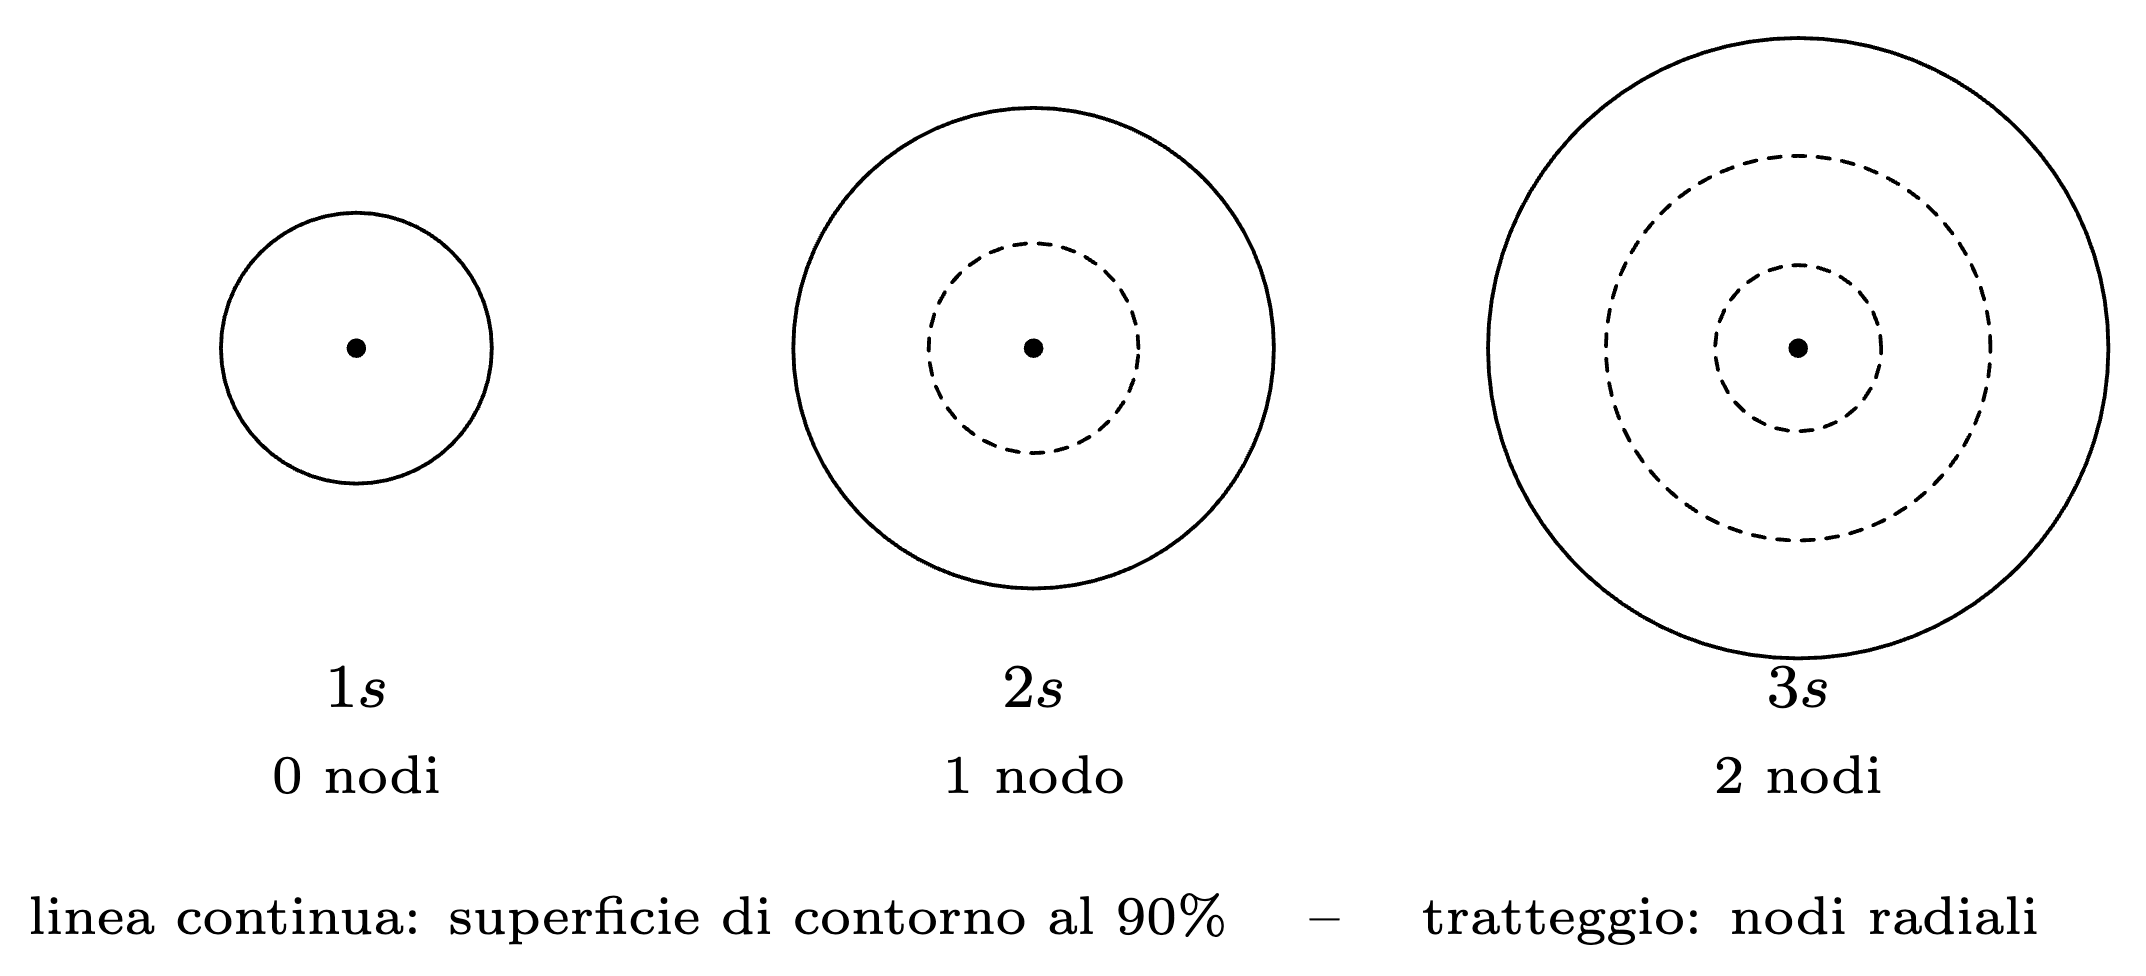
\includegraphics[width=0.9\linewidth]{foto/orbitali_s.png}
  \label{fig:etichetta}
\end{figure}

\newpage

\subsection{Orbitali p}

Gli orbitali con $l = 1$ esistono solo a partire da $n = 2$, essendo vincolati dalla condizione $l \leq n-1$. 
La loro funzione d'onda cambia segno passando da un semispazio all'altro e si annulla su un piano passante per il nucleo: tale piano nodale\mkeyword{piano nodale} separa i due lobi, che hanno forma identica ma fase opposta. Ne risulta la caratteristica geometria a manubrio.\\

\begin{figure}[h]
  \centering
  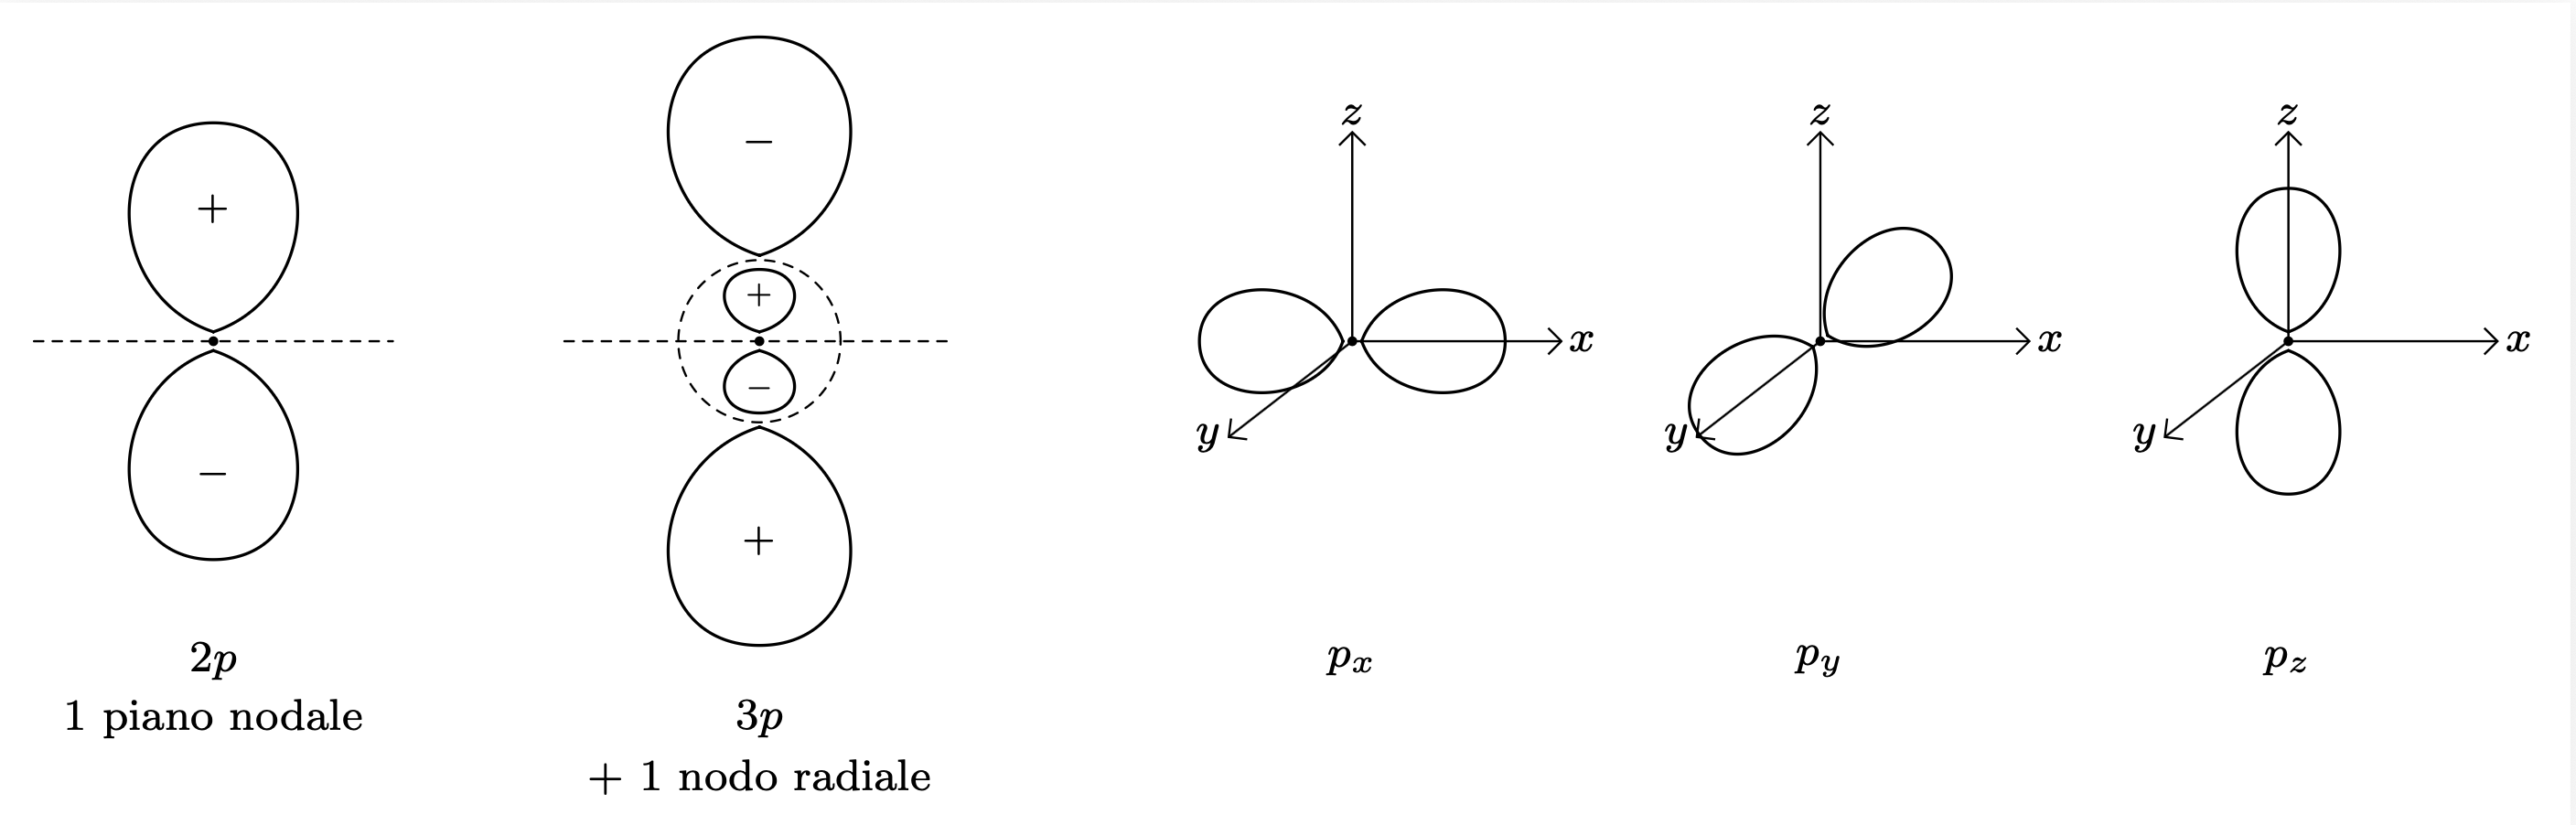
\includegraphics[width=1.0\linewidth]{foto/orbitali_p.png}
  \label{fig:etichetta}
\end{figure}

Poiché $m$ può assumere i tre valori $-1, 0, +1$, esistono tre orbitali p per ogni valore di $n$, orientati lungo i tre assi cartesiani e indicati con $p_x$, $p_y$ e $p_z$. 
Essi sono mutuamente ortogonali, nel senso che il prodotto scalare tra due funzioni d'onda distinte è nullo:

\begin{equation}
    \int \psi_i^* \psi_j \, d\tau = \delta_{ij}
    \label{eq:ortonormalita}
\end{equation}

È importante osservare che la parte angolare della funzione d'onda dipende solo da $l$ e da $m$, e non da $n$: la forma a manubrio è pertanto identica per $2p$, $3p$ e $4p$. 
Ciò che cambia al crescere di $n$ è la sola parte radiale, che si estende più lontano e acquista nodi sferici aggiuntivi in numero $n-2$; anche in questo caso il lobo più esterno risulta sempre il più grande.\\

\subsection{Orbitali d}

Gli orbitali con $l = 2$ esistono a partire da $n = 3$ e sono cinque, corrispondenti ai valori $m = -2, -1, 0, +1, +2$. 
Possiedono due piani nodali, in accordo con la regola generale secondo cui il numero di nodi angolari è pari a $l$, e presentano quindi quattro lobi. I lobi adiacenti hanno sempre fase opposta, il che è coerente con il fatto che un nodo separa regioni in cui la funzione d'onda cambia segno.\\


Quattro di essi -- $d_{xy}$, $d_{xz}$, $d_{yz}$ e $d_{x^2-y^2}$ - hanno la medesima forma a quadrifoglio e differiscono solo per l'orientamento: i primi tre hanno i lobi diretti tra gli assi, il quarto lungo gli assi. 
Il quinto, $d_{z^2}$, ha invece un aspetto marcatamente diverso, con due lobi lungo l'asse $z$ e un anello equatoriale. 
La differenza è però solo apparente: i cinque orbitali sono perfettamente equivalenti in energia, e $d_{z^2}$ è in realtà una combinazione lineare di due funzioni della stessa forma delle altre, resa necessaria dal fatto che con cinque funzioni non è possibile ottenere cinque orientamenti equivalenti nello spazio.\\

\subsection{Orbitali f e oltre}

Gli orbitali con $l = 3$ sono sette e possiedono tre piani nodali, con forme considerevolmente più complesse. Sono riempiti da elementi spesso pesanti e radioattivi.\\

Nulla vieta, dal punto di vista matematico, di proseguire con $l = 4$ e oltre: si otterrebbero nove orbitali g, e così via. Tali orbitali non trovano però riscontro chimico, poiché richiederebbero elementi con numero atomico talmente elevato da essere instabili. In pratica gli orbitali rilevanti sono s, p e d.\\

Va infine osservato che le forme qui descritte costituiscono una base per lo spazio delle funzioni d'onda, e che loro combinazioni lineari generano ulteriori insiemi di orbitali altrettanto legittimi. Su questa libertà si fonda il concetto di orbitale ibrido, che verrà introdotto a proposito della geometria molecolare.

\section{Riempimento degli orbitali}

L'energia di un orbitale dipende principalmente da n e in maniera minore da l, mentre il numero quantico m non influenza in alcun modo questa grandezza. Orbitali con stesso n e l ma diverso m prendono il nome di orbitali degeneri\mkeyword{orbitali degeneri}.\\

Un trucco pratico per confrontare l'energia tra vari orbitali è quello di considerare la somma tra n e l: l'orbitale con energia minore ha un numero più piccolo, mentre a parità di $n + l$ si ha che l'orbitale con energia più bassa è quello con n minore.\\

Tuttavia un modo migliore per ordinare gli orbitali secondo l'energia è con il seguente schema 

\begin{figure}[h]
  \centering
  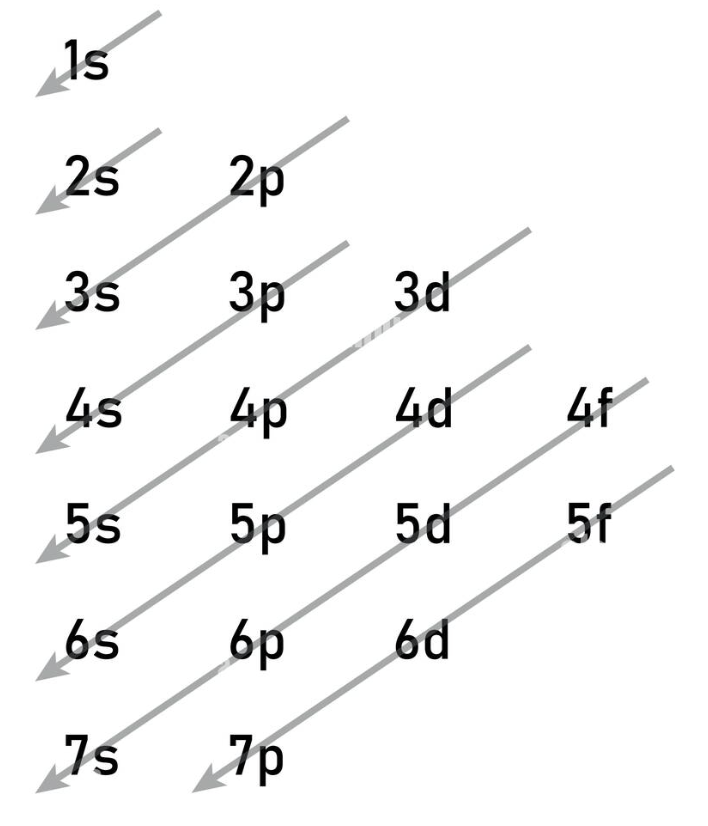
\includegraphics[width=0.4\linewidth]{foto/ordine_orbitali.png}
  \caption{Ordine di riempimento degli orbitali}
  \label{fig:etichetta}
\end{figure}

\newpage

\subsection{Principio di minima energia}

Il principio di minima energia presuppone che sia noto l'ordinamento energetico degli orbitali. Nell'atomo di idrogeno esso dipende dal solo numero quantico principale, come stabilito dalla \eqref{eq:energia_n}, e gli orbitali con lo stesso $n$ sono degeneri. 
Negli atomi polielettronici la degenerazione viene rimossa, e l'energia dipende sia da $n$ sia da $l$. Le cause sono due, di segno opposto.\\

La prima è l'attrazione esercitata dal nucleo, che cresce con il numero atomico: a parità di ogni altra condizione, una carica nucleare maggiore abbassa l'energia dell'orbitale e ne contrae l'estensione spaziale, stabilizzando il sistema.\\

La seconda è la repulsione fra gli elettroni, che agisce in senso contrario innalzando l'energia. 
Il suo effetto complessivo si descrive dicendo che gli elettroni interni \emph{schermano}\mkeyword{schermatura} quelli esterni, i quali risentono di una carica nucleare inferiore a quella reale. Si introduce allora la carica nucleare efficace\mkeyword{carica nucleare efficace}

\begin{equation}
    Z_{\text{eff}} = Z - \sigma
    \label{eq:zeff}
\end{equation}

dove $\sigma$ è la costante di schermo, e si tratta l'elettrone considerato come se fosse soggetto al solo campo di un nucleo di carica $Z_{\text{eff}}$.\\

La schermatura non è però la stessa per tutti gli elettroni. 
Un elettrone appartenente a un guscio interno scherma in modo assai più efficace di uno appartenente allo stesso sottolivello, poiché quest'ultimo si trova mediamente alla stessa distanza dal nucleo e per una parte del tempo si colloca più all'esterno. 
Ne segue che aggiungere un elettrone in un guscio interno abbassa sensibilmente $Z_{\text{eff}}$, mentre aggiungerlo nello stesso sottolivello la riduce solo di poco.\\

Resta da spiegare perché, a parità di $n$, l'energia dipenda da $l$. 
La causa è la penetrazione\mkeyword{penetrazione}: come mostrano le densità di probabilità radiali, un orbitale $2s$ possiede un lobo interno che lo porta in prossimità del nucleo, laddove un orbitale $2p$ ne è privo. L'elettrone $2s$ trascorre dunque una frazione non trascurabile del tempo all'interno della nuvola elettronica che lo scherma, risentendo in quegli istanti della carica nucleare pressoché completa. Il risultato è una $Z_{\text{eff}}$ maggiore e quindi un'energia minore, secondo l'ordinamento

\begin{equation}
    E_{ns} < E_{np} < E_{nd} < E_{nf}
    \label{eq:ordinamento}
\end{equation}

La \eqref{eq:ordinamento} è la ragione per cui il litio ha configurazione $1s^2 2s^1$ e non $1s^2 2p^1$, ed è più in generale ciò che determina l'ordine di riempimento e la struttura della tavola periodica. In alcuni casi la penetrazione è tale da invertire l'ordine atteso: l'orbitale $4s$, pur avendo $n$ maggiore, risulta più stabile del $3d$ e viene riempito per primo.

\newpage

\subsection{Principio di esclusione di Pauli}

Nella descrizione data finora ciascun elettrone è individuato da una quaterna di numeri quantici. Il principio di esclusione, enunciato da Pauli nel 1925, stabilisce un vincolo su quali quaterne possano coesistere in uno stesso atomo.\\

Due\mkeyword{principio di esclusione} elettroni appartenenti allo stesso atomo non possono avere tutti e quattro i numeri quantici uguali.\\

La conseguenza immediata è che ogni orbitale, essendo individuato dalla terna $(n,l,m)$, può contenere al massimo due elettroni, necessariamente con spin opposto.\\

Il principio non è però un postulato indipendente: esso discende dall'indistinguibilità degli elettroni. Poiché non è possibile etichettare una particella e seguirne l'identità, lo scambio di due elettroni non può modificare alcuna quantità osservabile, e in particolare la densità elettronica:

\begin{equation}
    |\psi(\mathbf{r_1},\mathbf{r_2})|^2 = |\psi(\mathbf{r_2},\mathbf{r_1})|^2
    \label{eq:indistinguibilita}
\end{equation}

La \eqref{eq:indistinguibilita} lascia due sole possibilità per la funzione d'onda, che può essere simmetrica o antisimmetrica rispetto allo scambio. 
L'esperienza mostra che per gli elettroni, e più in generale per tutte le particelle di spin semintero dette fermioni\mkeyword{fermioni}, vale il secondo caso:

\begin{equation}
    \psi(\mathbf{r_1},\mathbf{r_2}) = - \psi(\mathbf{r_2},\mathbf{r_1})
    \label{eq:antisimmetria}
\end{equation}

ed è questo il contenuto del principio di antisimmetria\mkeyword{principio di antisimmetria}. 
Si osservi che la \eqref{eq:antisimmetria} implica il principio di esclusione: se i due elettroni occupassero lo stesso stato, lo 
scambio delle coordinate lascerebbe la funzione d'onda inalterata e allo stesso tempo ne cambierebbe il segno, il che è possibile soltanto se essa è identicamente nulla. 
Uno stato con due elettroni identici semplicemente non esiste.\\

Va infine osservato che l'esistenza stessa della \eqref{eq:antisimmetria} comporta che la funzione d'onda di un sistema polielettronico dipenda dalle coordinate di tutti gli elettroni simultaneamente e non sia riducibile al prodotto di funzioni monoelettroniche. 
Parlare di un orbitale per ciascun elettrone costituisce pertanto un'approssimazione, per quanto assai utile.

\subsection{Regole per il riempimento degli orbitali}

Gli orbitali vengono riempiti seguendo queste regole:

\begin{itemize}
    \item Gli elettroni riempiono gli orbitali a più bassa energia disponibile. (Principio di minima energia)
    \item In ogni orbitale possono stare al massimo due elettroni, ma con spin cotrapposto. (Principio di esclusione di Pauli)
    \item Nel caso di orbitali degeneri, prima si riempiono tutti con un elettrone con spin $m_s = + 1/2$ e successivamente si aggiungono gli altri elettroni con spin $m_s = - 1/2$. (Regola di Hund)
\end{itemize}

\chapter{Proprietà degli elementi}

Le configurazioni elettroniche ricavate nel capitolo precedente non hanno soltanto valore descrittivo: da esse dipendono in modo diretto le proprietà fisiche e chimiche degli elementi. 
Poiché le configurazioni si ripetono con regolarità al crescere del numero atomico, anche tali proprietà mostrano un andamento periodico, ed è questa la ragione profonda dell'ordinamento della tavola periodica.

Tutti gli andamenti che seguono si spiegano mediante due sole grandezze già introdotte: la carica nucleare efficace $Z_{\text{eff}}$, che aumenta procedendo verso destra lungo un periodo, e il numero quantico principale $n$ degli elettroni di valenza, che aumenta scendendo lungo un gruppo.

\section{Raggio atomico}

Poiché la funzione d'onda non si annulla a distanza finita, l'atomo non possiede un confine definito e il raggio atomico\mkeyword{raggio atomico} non è una grandezza intrinseca, bensì una definizione operativa: si assume come raggio la metà della distanza minima alla quale due atomi dello stesso elemento possono avvicinarsi. 
Il valore dipende quindi dal tipo di legame considerato, ed è per questo che si distinguono un raggio covalente, uno metallico e uno di van der Waals. Per l'alluminio metallico si ha $r = 143 \ pm$, mentre per il cloro legato covalentemente si ha $r = 100 \ pm$.

Il raggio atomico cresce scendendo lungo un gruppo e procedendo verso sinistra lungo un periodo. Le due tendenze hanno cause distinte.

Scendendo lungo un gruppo gli elettroni di valenza occupano orbitali con $n$ crescente, i quali si estendono progressivamente più lontano dal nucleo; gli elettroni interni, che aumentano di numero, schermano efficacemente la carica nucleare, sicché l'aumento di $Z$ non riesce a compensare l'aumento di $n$.

Procedendo verso destra lungo un periodo, al contrario, gli elettroni vengono aggiunti al medesimo guscio e si schermano fra loro in modo assai poco efficace, mentre la carica nucleare aumenta di un'unità per ogni elemento. 
Ne risulta un aumento di $Z_{\text{eff}}$ che contrae progressivamente l'orbitale: il raggio del litio è maggiore di quello del berillio, benché entrambi abbiano gli elettroni di valenza in $2s$. È un risultato controintuitivo, giacché l'atomo si rimpicciolisce pur acquistando elettroni.

I raggi minori si riscontrano quindi nei gas nobili, che occupano l'estremità destra di ciascun periodo.

\newpage

\section{Raggio ionico}

Uno ione possiede un numero di elettroni diverso da quello dell'atomo neutro, e non è pertanto lecito attribuirgli il raggio atomico. Si definisce allora un raggio ionico\mkeyword{raggio ionico}, ricavato dalle distanze interioniche misurate nei cristalli.

Un catione è sempre più piccolo dell'atomo da cui deriva: la perdita di elettroni riduce la repulsione interelettronica e, se l'elettrone rimosso era l'unico del guscio più esterno, ne elimina uno per intero. Un anione è invece sempre più grande, poiché l'aggiunta di elettroni aumenta la repulsione senza alcuna variazione della carica nucleare. Il sodio passa da $186 \ pm$ a $102 \ pm$ nella forma $Na^+$, mentre il cloro passa da $100 \ pm$ a $181 \ pm$ nella forma $Cl^-$.

\section{Energia di ionizzazione}

Si definisce energia di prima ionizzazione\mkeyword{energia di ionizzazione} l'energia necessaria a rimuovere un elettrone da un atomo neutro isolato allo stato gassoso.

\begin{equation}
    X_{(g)} + E_i \longrightarrow X^+_{(g)} + e^-
    \label{eq:ionizzazione}
\end{equation}

Il processo è sempre endotermico, poiché l'elettrone è legato al nucleo eoccorre fornire energia per allontanarlo indefinitamente.

L'energia di ionizzazione cresce procedendo verso destra lungo un periodo, per effetto dell'aumento di $Z_{\text{eff}}$, e diminuisce scendendo lungo un gruppo, poiché l'elettrone da rimuovere si trova mediamente più lontano dal nucleo. 
I valori massimi si riscontrano quindi nei gas nobili e i minimi nei metalli alcalini: si tratta dello stesso andamento del raggio atomico, percorso in senso inverso.

L'andamento lungo il periodo presenta tuttavia due irregolarità sistematiche, che costituiscono una conferma indipendente della struttura elettronica.
Passando dal gruppo $2A$ al gruppo $3A$ l'energia diminuisce anziché crescere, perché l'elettrone da rimuovere non appartiene più a un orbitale $s$ ma a un orbitale $p$, meno penetrante e quindi meno legato. 
Analogamente, passando dal gruppo $5A$ al gruppo $6A$ si osserva una diminuzione, poiché il sesto elettrone deve appaiarsi in un orbitale $p$ già occupato e risente di una repulsione interelettronica aggiuntiva: la configurazione $np^3$, con i tre orbitali degeneri occupati da elettroni a spin parallelo secondo la regola di Hund, è particolarmente stabile.

Le energie di ionizzazione successive sono sempre crescenti, giacché ciascun elettrone viene strappato a uno ione di carica via via maggiore. 
L'aumento è graduale finché si rimuovono elettroni di valenza, mentre si osserva un salt di energia assai marcato nel momento in cui si comincia a intaccare un guscio interno completo. La posizione di tale salto individua il numero di elettroni di valenza dell'elemento, e costituisce una delle evidenze sperimentali più dirette dell'esistenza dei gusci.

\newpage

\section{Affinità elettronica}

Si definisce affinità elettronica\mkeyword{affinità elettronica} l'energia in gioco quando un atomo neutro isolato allo stato gassoso acquista un elettrone.

\begin{equation}
    X_{(g)} + e^- \longrightarrow X^-_{(g)}
    \label{eq:affinita}
\end{equation}

A differenza della \eqref{eq:ionizzazione}, il processo può essere sia esotermico sia endotermico. Negli alogeni, ai quali manca un solo elettrone per completare l'ottetto, esso è fortemente esotermico e l'affinità elettronica raggiunge i valori massimi in valore assoluto. 
Nei gas nobili, viceversa, l'elettrone dovrebbe collocarsi in un guscio nuovo e il processo risulta endotermico.

L'affinità elettronica cresce in generale procedendo verso destra lungo un periodo, con eccezioni in corrispondenza delle configurazioni particolarmente stabili $ns^2$, $ns^2np^3$ e $ns^2np^6$, per le quali l'elettrone aggiuntivo sarebbe fortemente destabilizzato.

\section{Metalli, non metalli e semimetalli}

Le proprietà finora esaminate permettono di classificare gli elementi in tre categorie, separate nella tavola periodica da una linea diagonale che scende dal boro verso l'astato.\\

I metalli\mkeyword{metalli} occupano la parte sinistra e centrale della tavola. Sono caratterizzati da energie di ionizzazione basse, e tendono pertanto a cedere elettroni formando cationi in soluzione acquosa. 
Allo stato solido riflettono la luce, sono duttili e malleabili e conducono bene la corrente elettrica e il calore, proprietà tutte riconducibili alla delocalizzazione degli elettroni di valenza nel reticolo. 
Il carattere metallico è massimo nei gruppi $1A$ e $2A$, con la sola eccezione dell'idrogeno, e cresce scendendo lungo un gruppo; tutti gli elementi di transizione sono metalli.\\

I non metalli\mkeyword{non metalli} occupano la parte destra della tavola.
Avendo elevata affinità elettronica, acquistano elettroni quando reagiscono con i metalli.

Allo stato solido sono fragili e non malleabili, e sono in genere cattivi conduttori. \\

I semimetalli\mkeyword{semimetalli}, o metalloidi, si collocano lungo la linea di separazione e presentano proprietà intermedie. 
Il silicio, ad esempio, ha aspetto metallico ma è fragile, e la sua conducibilità è intermedia fra quella dei metalli e quella degli isolanti: su questa proprietà si fonda l'intera elettronica a semiconduttori.

\subsection{Gruppo 1A: metalli alcalini}

Gli elementi del primo gruppo possiedono configurazione di valenza $ns^1$ e cedono con grande facilità l'unico elettrone esterno, essendo la loro energia di prima ionizzazione la più bassa dell'intero periodo. 
Nei composti compaiono pertanto sempre come cationi monovalenti $M^+$\mkeyword{metalli alcalini}. 
Allo stato elementare sono metalli morbidi e la loro reattività aumenta scendendo lungo il gruppo, poiché l'elettrone di valenza si trova progressivamente più lontano dal nucleo.\\

\subsection{Gruppo 2A: metalli alcalino-terrosi}

La configurazione di valenza $ns^2$ comporta la cessione di due elettroni e la formazione di cationi bivalenti $M^{2+}$\mkeyword{metalli alcalino-terrosi}. 
Rispetto agli alcalini essi sono più duri e meno reattivi, giacché la maggiore carica nucleare rende più difficoltosa la rimozione degli elettroni; anche in questo caso la reattività cresce scendendo lungo il gruppo.\\

\subsection{Idrogeno}

L'idrogeno occupa una posizione anomala nella tavola periodica. La configurazione $1s^1$ lo accomunerebbe ai metalli alcalini, ma il fatto che gli manchi un solo elettrone per completare il guscio lo avvicina agli alogeni, e in effetti ne condivide alcuni comportamenti.\mkeyword{idrogeno}\\

\subsection{Gruppo 6A: calcogeni}

Il sesto gruppo illustra con particolare chiarezza l'aumento del carattere metallico lungo un gruppo: l'ossigeno è un non metallo, il tellurio un semimetallo e il polonio un metallo a tutti gli effetti.\mkeyword{calcogeni}\\

L'ossigeno esiste in due forme allotropiche, la molecola biatomica $O_2$ e l'ozono $O_3$, quest'ultimo meno stabile e ottenibile dalla prima solo fornendo energia

\begin{equation}
    3O_{2(g)} \longrightarrow 2O_{3(g)} \qquad \Delta H = + 284,6 \ kJ
    \label{eq:ozono}
\end{equation}

condizione che si realizza nell'alta atmosfera per effetto della radiazione ultravioletta. Data l'elevata elettronegatività, l'ossigeno è un potente agente ossidante e presenta numero di ossidazione $-2$ nella gran parte dei composti, come nell'acqua, e $-1$ nei perossidi come $H_2O_2$. Lo zolfo, meno elettronegativo, compare nei composti binari come ione solfuro $S^{2-}$.

\subsection{Gruppo 7A: alogeni}

Gli alogeni possiedono configurazione $ns^2np^5$ e necessitano di un solo elettrone per completare l'ottetto: la loro affinità elettronica è pertanto la più elevata in valore assoluto\mkeyword{alogeni}. La reazione caratteristica è la riduzione a ione alogenuro

\begin{equation}
    X_2 + 2e^- \longrightarrow 2X^-
    \label{eq:alogenuro}
\end{equation}

Allo stato elementare formano molecole biatomiche $X_2$, il cui stato di aggregazione varia con la massa molecolare: fluoro e cloro sono gas, il bromo è liquido e lo iodio è solido, in conseguenza dell'aumento delle forze di London con il numero di elettroni. 
Il fluoro è fra le sostanze più reattive in assoluto, e la reattività diminuisce scendendo lungo il gruppo.

\subsection{Gruppo 8A: gas nobili}

I gas nobili possiedono i sottolivelli $s$ e $p$ completamente riempiti, configurazione che comporta la massima energia di ionizzazione e un'affinità elettronica praticamente nulla\mkeyword{gas nobili}. 
Non avendo alcuna tendenza né a cedere né ad acquistare elettroni, sono chimicamente inerti e si presentano monoatomici allo stato elementare, unico caso fra tutti gli elementi.\\

L'inerzia non è tuttavia assoluta: gli elementi più pesanti del gruppo, per i quali l'energia di ionizzazione è sensibilmente minore, formano composti con i soli elementi più elettronegativi, come nel caso di $XeF_4$ e $XeOF_4$.

\chapter{Legami}

Per raggiungere la configurazione più stabile, che corrisponde a quella dei gas nobili ($s^2p^6$), gli atomi condividono o scambiano elettroni attraverso quelli che prendenono il nome di legami. 

Esistono 3 tipi di legami chimici

\begin{itemize}
    \item legame ionico: attrazione elettrostatica tra ioni di segno opposto
    \item legame covalente: compartecipazione di elettroni tra due atomi 
    \item legame metallico: compartecipazione di elettroni tra un gran numero di atomi
\end{itemize}

Gli elettroni nel guscio più esterno, coinvolti nei legami, prendono il nome di elettroni di valenza\mkeyword{elettroni di valenza}.\\

Un'importante regola empirica è la regola dell'ottetto\mkeyword{regola dell'ottetto}, formulata da Lewis nel 1917, secondo cui quando un atomo possiede il livello elettronico esterno completo (detto guscio di valenza), in genere costituito da 8 elettroni, esso è in una particolare condizione di stabilità energetica e tende a non formare ulteriori legami. 

\section{Legame ionico}

Il modo più semplice per conseguire la configurazione a ottetto consiste nel trasferimento completo di uno o più elettroni da un atomo all'altro, con formazione di ioni di carica opposta che si attraggono elettrostaticamente: si parla in tal caso di legame ionico\mkeyword{legame ionico}. 
Esso si instaura fra elementi di elettronegatività assai diversa, tipicamente un metallo e un non metallo, come nella formazione del cloruro di sodio

\begin{equation}
    Na_{(s)} + \frac{1}{2} Cl_{2(g)} \longrightarrow NaCl_{(s)}
    \label{eq:formazione_nacl}
\end{equation}

Va osservato che la formazione degli ioni isolati allo stato gassoso è nel complesso endotermica, poiché l'affinità elettronica del cloro non compensa l'energia di ionizzazione del sodio. Il processo complessivo risulta esotermico soltanto grazie al successivo impacchettamento degli ioni nel reticolo cristallino, che libera una quantità di energia assai maggiore.\\

Non esiste dunque una molecola di $NaCl$: il composto è costituito da un reticolo tridimensionale nel quale ciascuno ione $Na^+$ è circondato da sei ioni $Cl^-$ e viceversa, secondo la disposizione più compatta possibile. 
La formula chimica esprime pertanto un rapporto stechiometrico e non un'entità discreta.\\

Si definisce energia reticolare\mkeyword{energia reticolare} l'energia richiesta per separare una mole di composto ionico solido negli ioni corrispondenti allo stato gassoso.


L'energia reticolare dipende dalla carica e dalle dimensioni degli ioni: cresce al crescere delle cariche, che compaiono come prodotto, e al diminuire della distanza interionica.\\

\subsection{Costante di Madelung}

Per ricavarne l'espressione si consideri dapprima un reticolo unidimensionale di ioni alternati a distanza $r_0$. 

\begin{figure}[h]
  \centering
  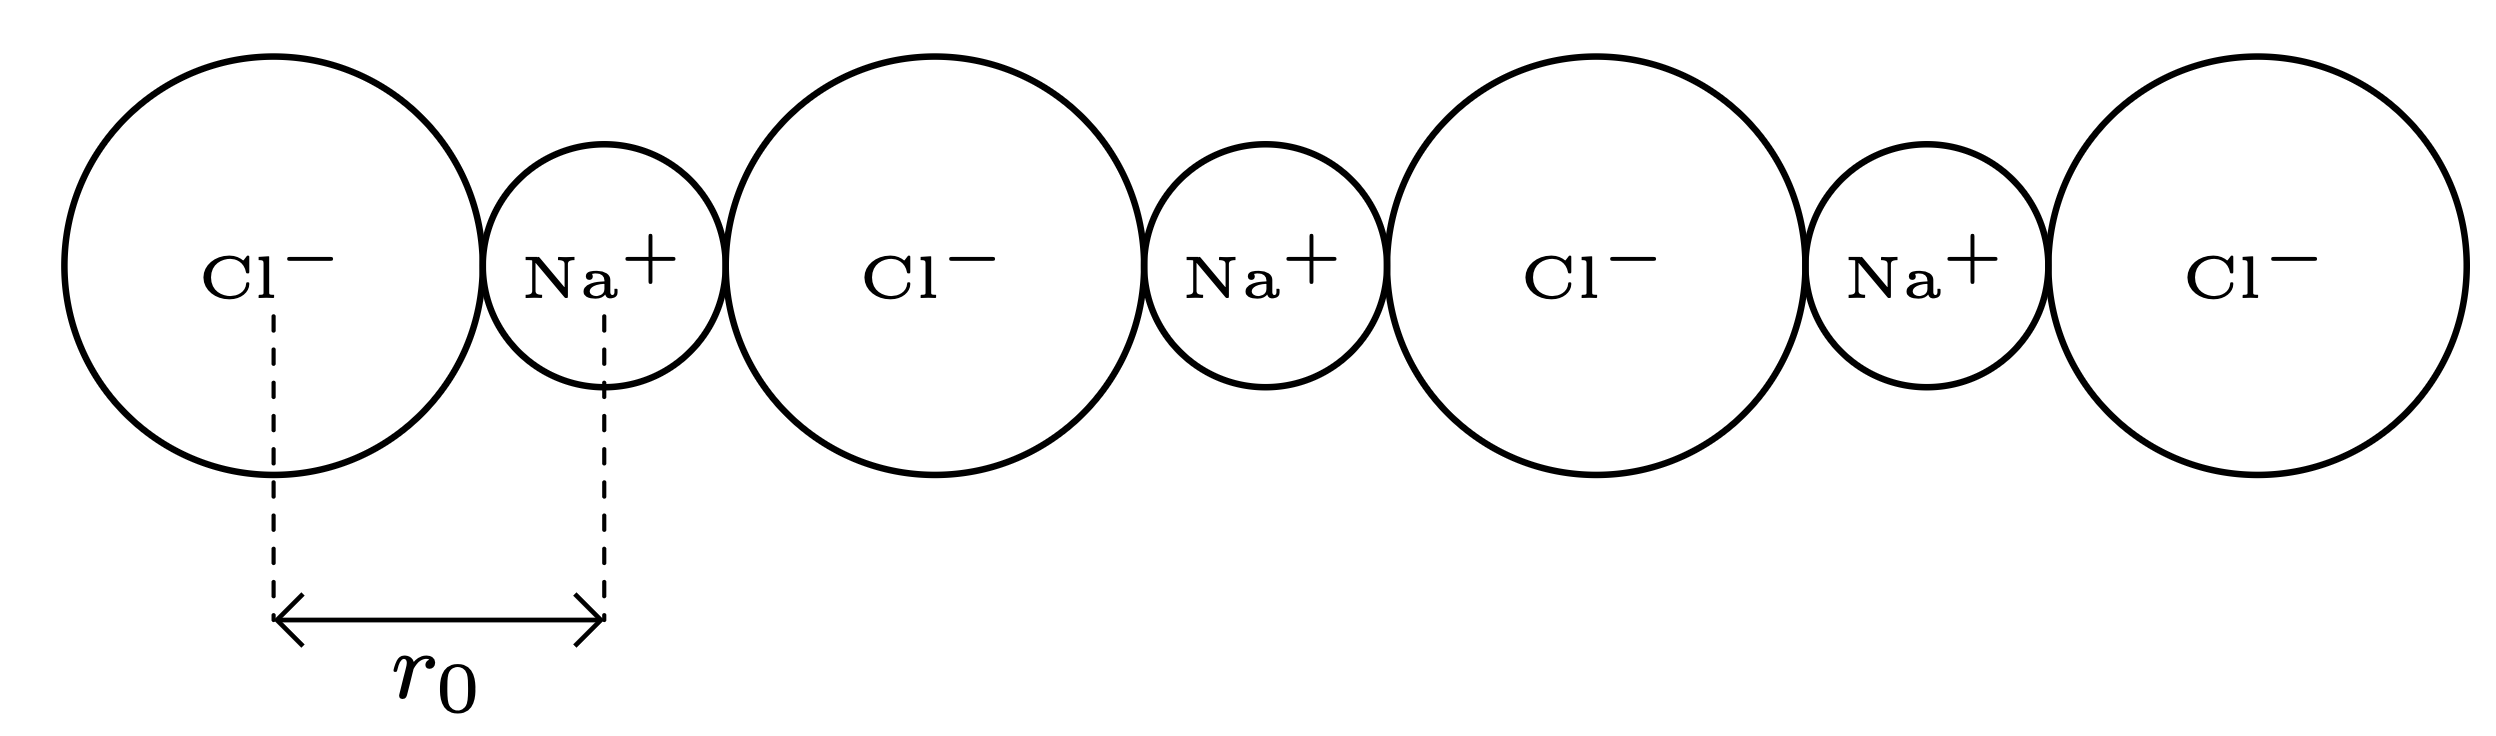
\includegraphics[width=0.7\linewidth]{foto/reticolo_1D.png}
  \caption{reticolo 1D}
  \label{fig:etichetta}
\end{figure}

Sommando i contributi coulombiani di tutti gli ioni si ottiene una serie a segni alterni, il cui valore conduce a

\begin{equation}
    E = - \frac{z_1 z_2 e^2}{4\pi\varepsilon_0 r_0} \cdot 2\ln 2
    \label{eq:madelung_1d}
\end{equation}

Nel caso tridimensionale la somma dipende dalla particolare geometria del reticolo e non è esprimibile in forma chiusa; si scrive allora

\begin{equation}
    E = - \frac{z_1 z_2 e^2}{4\pi\varepsilon_0 r_0} \cdot M
    \label{eq:madelung_3d}
\end{equation}

dove $M$ prende il nome di costante di Madelung\mkeyword{costante di Madelung} e dipende esclusivamente dalla disposizione geometrica degli ioni. Per il cloruro di sodio si ha $M = 1,7476$.\\

Il modello puramente elettrostatico descritto dalla \eqref{eq:madelung_3d} non è tuttavia completo: essendo l'energia proporzionale a $-1/r_0$, esso prevedrebbe un collasso del reticolo su sé stesso. 
Occorre aggiungere un termine repulsivo a corto raggio, di origine quantistica e riconducibile al principio di esclusione, che si oppone alla compenetrazione delle nubi elettroniche e determina la distanza di equilibrio $r_0$.\\

Le proprietà macroscopiche dei composti ionici discendono direttamente da questa struttura. Essi sono altofondenti, poiché fondere il cristallo richiede di vincere l'intera energia reticolare, e sono isolanti allo stato solido, dove gli ioni sono vincolati alle rispettive posizioni, mentre conducono la corrente se fusi o disciolti in acqua, condizioni nelle quali gli ioni acquistano libertà di movimento. Sono infine fragili: una sollecitazione esterna che faccia scorrere un piano reticolare rispetto all'adiacente porta a contatto ioni di carica uguale, e la repulsione che ne consegue provoca la frattura netta del cristallo.\\


\end{document}